\chapter{Introduzione}

\section{Scopo del Documento}
Con questo documento vogliamo fornire una descrizione dettagliata del prodotto, andando ad analizzare i singoli
requisiti, individuati tramite la presentazione del capitolato e gli incontro con il proponente, grazie ai quali
possiamo capire i vari attori del sistema e illustrare i diversi casi d'uso relativi al prodotto software.
\newline
Inoltre questo documento offre anche supporto ai progettisti, poiché fornisce una chiara idea sui vari componenti del programma.

\section{Introduzione ai Casi d'Uso}
\subsection{Scopo}
L'obiettivo è quello di elencare tutti i casi d'uso individuati dl gruppo, per poterli analizzare uno a uno e capirli al meglio.
\newline
Per ogni caso d'uso troviamo:
\begin{itemize}
  \item \textbf{Descrizione}: breve descrizione del caso d'uso;
  \item \textbf{Attore primario}: chi può eseguire questa azione;
  \item \textbf{Precondizioni}: lo stato del programma prima del caso d'uso;
  \item \textbf{Postcondizioni}: lo stato del programma in seguito al caso d'uso;
  \item \textbf{Scenario principale}: le azioni svolte prima, durante e dopo il caso d'uso.
\end{itemize}

\subsection{Attori}
Il prodotto verrà utilizzato solo per scopo di sorveglianza interno, senza il bisogno di figure particolari per il suo funzionamento
come un amministratore o un utente registrato, perciò sarà presente solo un attore all'interno del sistema: un utente generico, che avrà accesso a tutte
le funzionalità del prodotto. 
\begin{figure}[h]
  \centering
  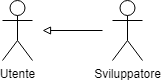
\includegraphics[width=0.08\textwidth]{attori}
  \caption{Attori del sistema}
\end{figure}

\section{Riferimenti}
\subsection{Riferimenti normativi}
\begin{itemize}
  \item \textit{Norme di Progetto}
  \item Capitolato d'appalto C5 - Zucchetti S.p.A.: Login Warrior \\
  \url{https://www.math.unipd.it/~tullio/IS-1/2021/Progetto/C5.pdf}
\end{itemize}

\subsection{Riferimenti informativi}
\begin{itemize}
  \item Slide T7 - Corso di Ingegneria del Software - Analisi dei requisiti \\
  \url{https://www.math.unipd.it/~tullio/IS-1/2021/Dispense/T07.pdf}
  \item Slide P2 - Corso di Ingegneria del Software - Diagrammi delle clasi \\
  \url{https://www.math.unipd.it/~rcardin/swea/2021/Diagrammi%20delle%20Classi_4x4.pdf}
  \item Slide P4 - Corso di Ingegneria del Software - Diagrammi dei casi d'uso \\
  \url{https://www.math.unipd.it/~rcardin/swea/2022/Diagrammi%20Use%20Case.pdf}
  \item Slide P4 - Corso di Ingegneria del Software - Diagrammi di attività \\
  \url{https://www.math.unipd.it/~rcardin/swea/2022/Diagrammi%20di%20Attivit\%C3\%A0.pdf}  % \%C3\%A0 serve per inserire la à nel link
  \item Slide P5 - Corso di Ingegneria del Software - Diagrammi di sequenza \\
  \url{https://www.math.unipd.it/~rcardin/swea/2022/Diagrammi%20di%20Sequenza.pdf}
\end{itemize}
